\chapter{Entwurfsmuster}
\section{Factory Method}
Das Entwurfsmuster der Factory Method wird von der EntryFactory umgesetzt. Um ein Entry aus den Standarddatentypen zu erzeugen hat die EntryFactory zwei verschiedene statische Factorymethoden. Die Methode \textit{createEntry} nimmt alle notwendigen Daten als Standarddatentyp, also die EntryId als unsigned int, den EntryName, Login und EncryptedPassword als string, und erzeugt daraus die notwendigen Value Objects, um letztendlich den Entry zu erzeugen. Die Methode \textit{createEntryFromPlaintext} hingegen nimmt ebenfalls alle vier notwendigen Parameter als Standarddatentypen entgegen, geht jedoch davon aus, dass das Passwort nicht verschlüsselt ist, weshalb vorerst ein PlaintextPassword aus dem übergebenen String erzeugt wird, das dann an den PasswordEncryptor Domain Service übergeben wird, um ein EncryptedPassword zu erzeugen. Schließlich wird auch hier ein Entry aus den erzeugten Value Objects erzeugt und zurückgegeben. Die EntryFactory vereinfacht also das Erzeugen von Entries dadurch, dass nicht immer erst alle vier Value Objects, die notwendig sind um den Konstruktor des Entrys aufzurufen, erzeugt werden müssen, sondern direkt als Standarddatentyp übergeben werden können und die Factory diese Umwandlung intern vornimmt. Eine Visualisierung der EntryFactory in Form eines UML-Diagramms kann in \autoref{fig:EntryFactory} betrachtet werden.\\

\begin{figure}[ht]
	\centering
	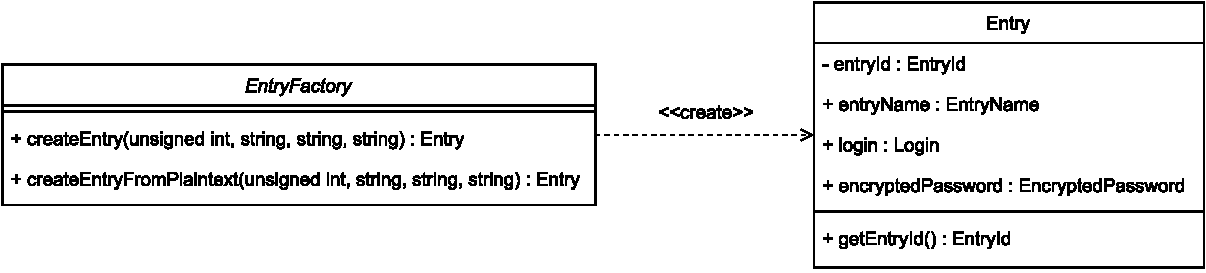
\includegraphics[width=1.0\textwidth]{Bilder/EntryFactory.pdf}
	\caption{UML-Diagramm EntryFactory}
	\label{fig:EntryFactory}
\end{figure}
